\documentclass[twocolumn]{autart}

\usepackage{graphicx}          % Include this line if your 
                               % document contains figures,
%\usepackage[dvips]{epsfig}    % or this line, depending on which
                               % you prefer.

\begin{document}

\begin{frontmatter}
%\runtitle{Insert a suggested running title}  % Running title for regular 
                                              % papers but only if the title  
                                              % is over 5 words. Running title 
                                              % is not shown in output.

\title{Archaeology 4.0: \protect\\ Archaeology in the Third Era of Computing}
                                               

\author[FT]{Florian Thiery}\ead{rse@fthiery.de}

\address[FT]{Research Software Engineer, Mainz, Germany}  % Please supply                                              

          
\begin{keyword}                           % Five to ten keywords,  
Cicero; Catiline; orations.               % chosen from the IFAC 
\end{keyword}                             % keyword list or with the 
                                          % help of the Automatica 
                                          % keyword wizard


\begin{abstract}                         

Lorem ipsum dolor sit amet, consetetur sadipscing elitr, sed diam nonumy eirmod tempor invidunt ut labore et dolore magna aliquyam erat, sed diam voluptua. At vero eos et accusam et justo duo dolores et ea rebum. Stet clita kasd gubergren, no sea takimata sanctus est Lorem ipsum dolor sit amet. Lorem ipsum dolor sit amet, consetetur sadipscing elitr, sed diam nonumy eirmod tempor invidunt ut labore et dolore magna aliquyam erat, sed diam voluptua. At vero eos et accusam et justo duo dolores et ea rebum. Stet clita kasd gubergren, no sea takimata sanctus est Lorem ipsum dolor sit amet. Lorem ipsum dolor sit amet, consetetur sadipscing elitr, sed diam nonumy eirmod tempor invidunt ut labore et dolore magna aliquyam erat, sed diam voluptua. At vero eos et accusam et justo duo dolores et ea rebum. Stet clita kasd gubergren, no sea takimata sanctus est Lorem ipsum dolor sit amet. 

\end{abstract}

\end{frontmatter}

\section{Archaeological Evolution}

Today, in 2019 we are living in the centre of the Digital Transformation era. The digital transformation affects all kind of 'humanoid' and 'machine' communities: individuals and society, state, companies and science (research/teaching). In archaeology, researcher develop and use new digital technologies. This results in positive effects on science and archaeology itself. The state promotes (e.g. funding by the Federal Ministry of Education and Research - BMBF) and uses these digital technologies and serves as a regulator. Also the society is using more and more digital technologies. Companies are developing and using new digital technologies as well.

\begin{figure}[!htb]
\begin{center}
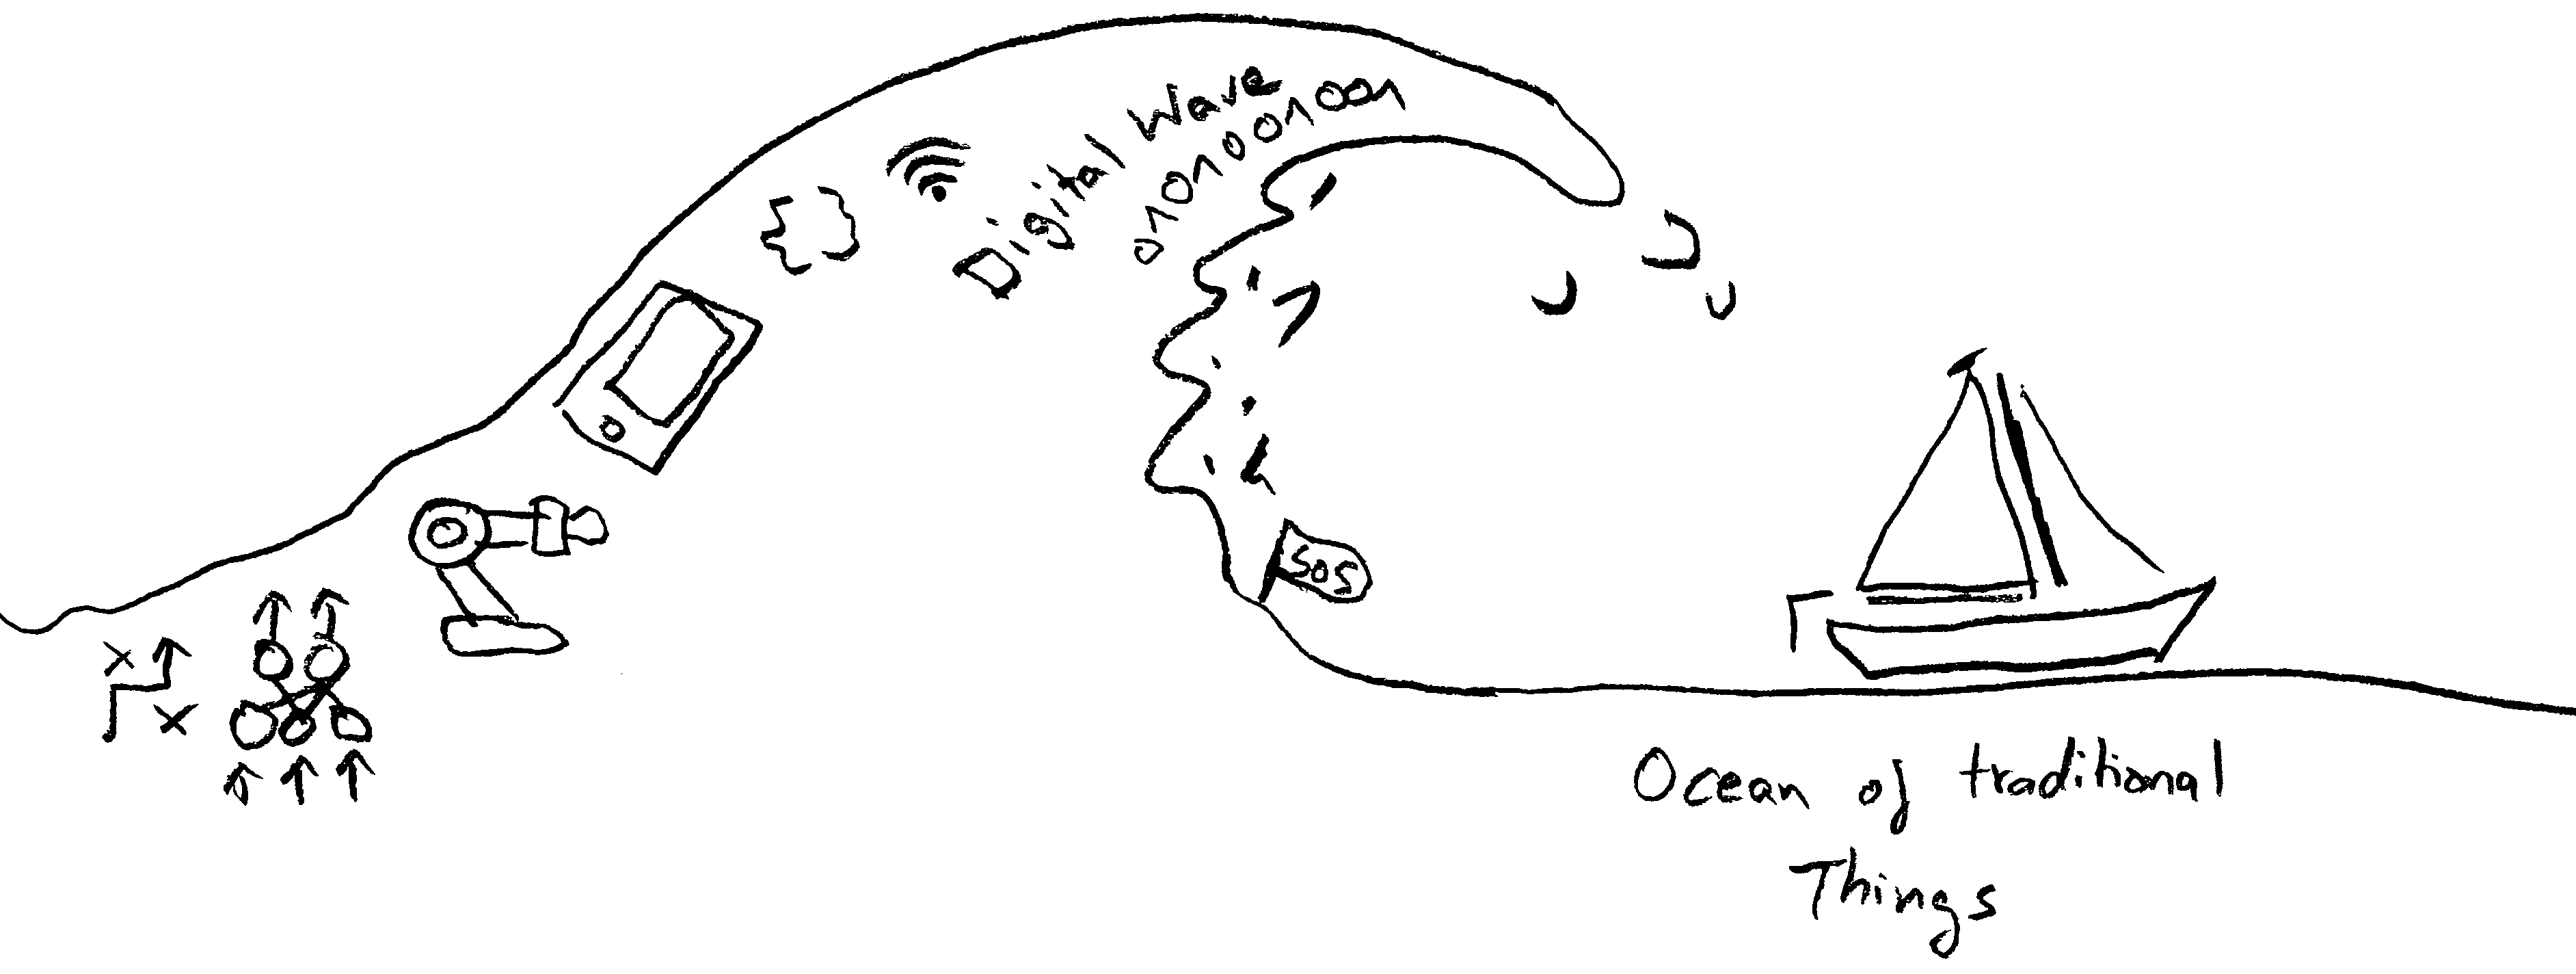
\includegraphics[width=8cm]{Digital_Wave_and_the_Ocean_of_Traditional_Things.png}
\caption{The Digital and the Ocean of Traditional Things, Florian Thiery [CC BY 4.0]}
\label{figdigitalwave}
\end{center}
\end{figure}

Thus, science and archaeology should seek collaboration with companies to positively influence the state and society through digital technologies. But does the digital wave overtake us? (Fig.~\ref{figdigitalwave}) We should surf the wave! On a first wave of digitalisation we have already recorded, saved, transmitted and processed machine-readable data via internet and cloud computing technologies. Furthermore, on the second wave of digitalisation we have to analyse, enhance and use these research data in active ways as machine-interpretable data using artificial intelligence and machine learning.

While surfing the waves, we actively experience the evolution of archaeology from analogue data to Knowledge Graph Computing. That is what I will call Archaeology 4.0 (Fig.~\ref{figa40pyramid}).

\begin{figure}[!htb]
\begin{center}
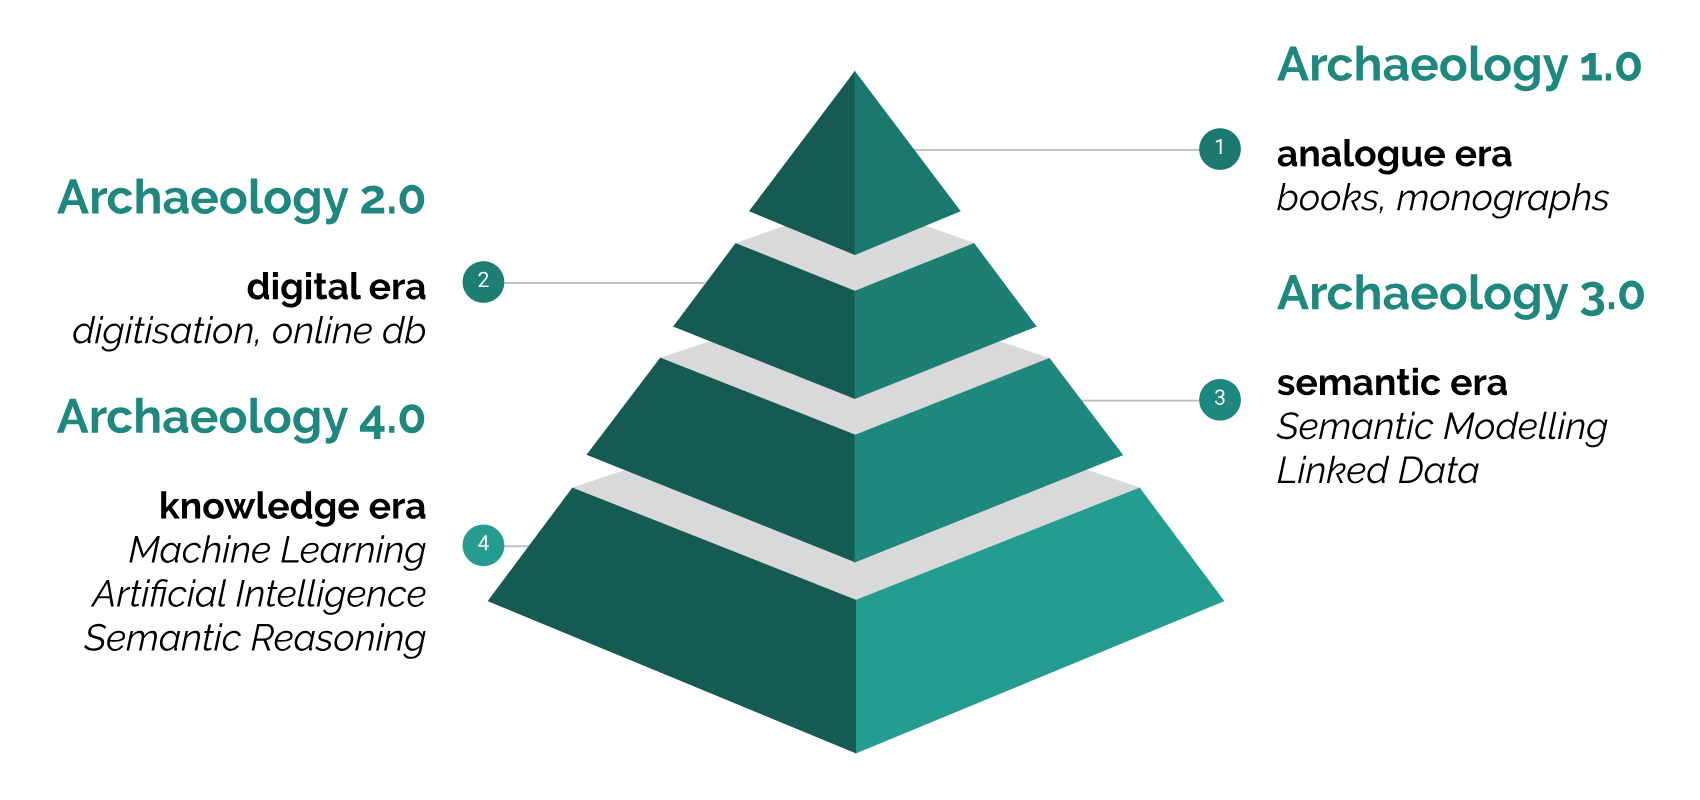
\includegraphics[width=8cm]{Archaeology_40.png}    % The printed column  
\caption{Archaelogy 4.0, Florian Thiery [CC BY 4.0]}  % width is 8.4 cm.
\label{figa40pyramid}                                 % Size the figures 
\end{center}                                 % accordingly.
\end{figure}

Archaeologal Sciences fulfilled a digital transformation from an 'analogous science' to modern digital science of humanities. Starting from an \textit{analogue era} (Archaeology 1.0), in which research data was kept in books and monographs, across the \textit{digital era} (Archaeology 2.0) in which digitisation progresses and data are published on the WWW, to a \textit{semantic era} (Archaeology 3.0), where semantic modelling and publication of Linked Data prevail, we end up in a \textit{knowledge era} (Archaeology 3.0), in which the analysis and the creation of new knowledge through a machine results.

\subsection{Archaeology 1.0}

\begin{figure}[!htb]
\begin{center}

\includegraphics[height=2cm]{a10.png}    % The printed column  
\caption{Archaelogy 1.0 Symbol, pixabay [Pixabay License]}  % width is 8.4 cm.
\label{figa10symbol}                                 % Size the figures 
\end{center}                                 % accordingly.
\end{figure}

I will call the era of non digital things ('analogue') the \textit{analogue era}. Research, and its underlying data, was published in printed books and monographs. Data access was only possible via active visiting libraries or complicated interlibrary loan. Research Data was not 'OPEN' at this time, because it was a privilege of an individual. 

\subsection{Archaeology 2.0}

\begin{figure}[!htb]
\begin{center}
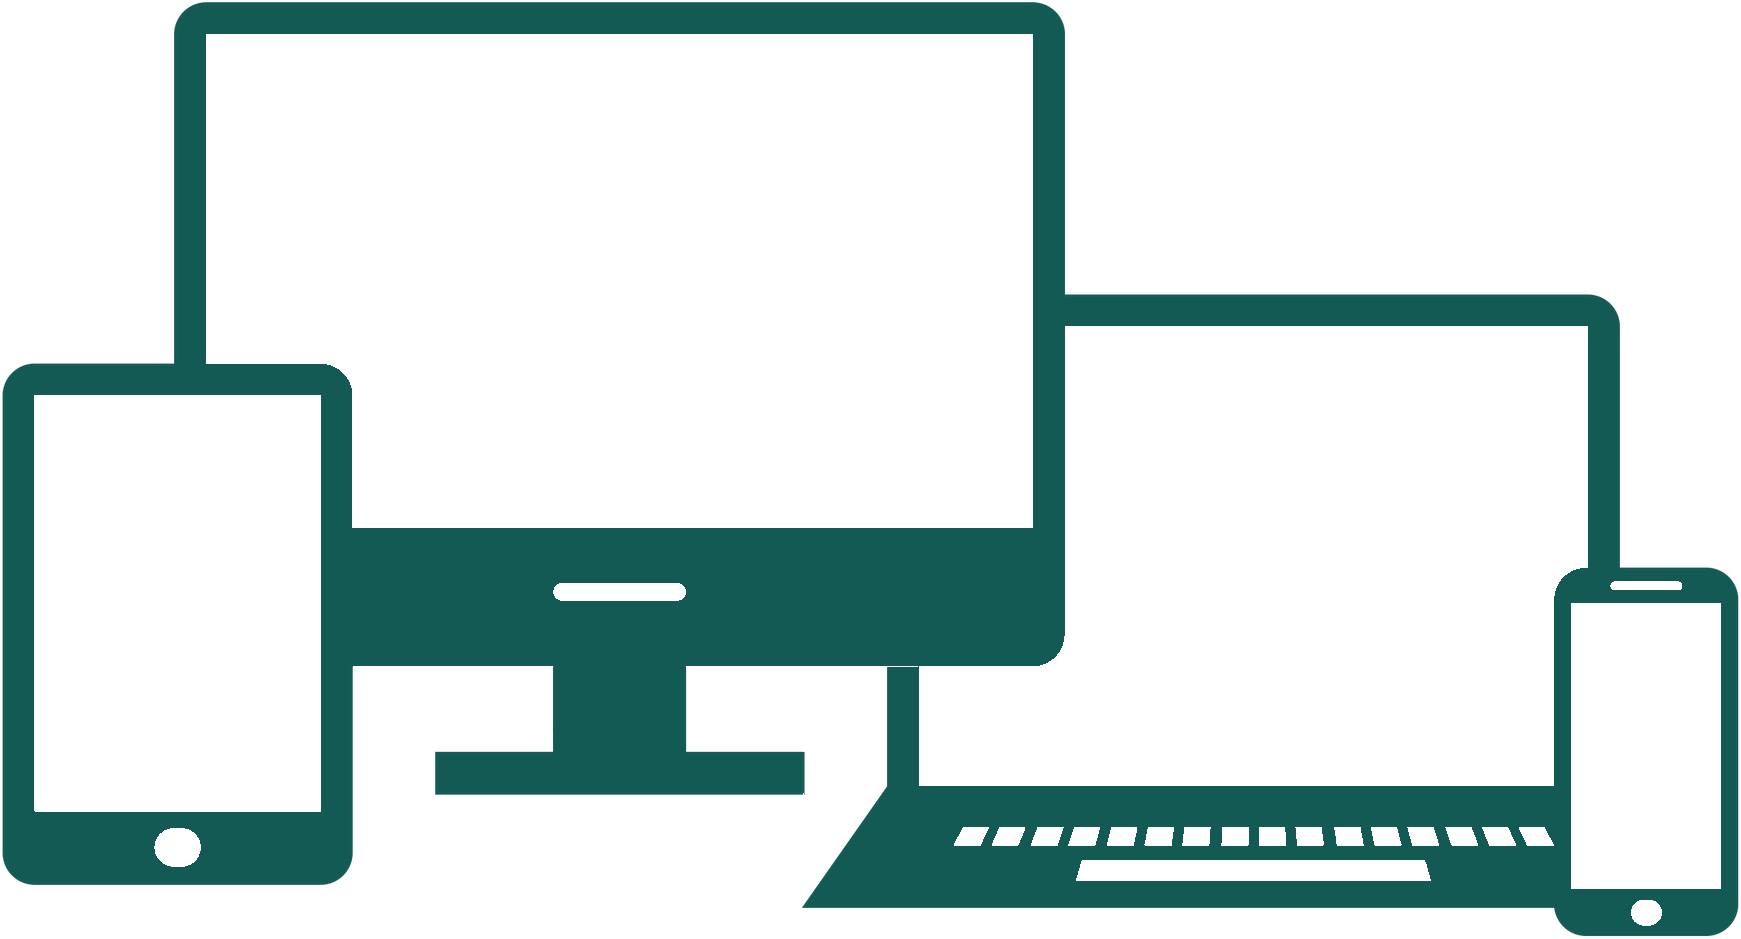
\includegraphics[height=2cm]{a20.png}    % The printed column  
\caption{Archaelogy 2.0 Symbol, pixabay [Pixabay License]}  % width is 8.4 cm.
\label{figa20symbol}                                 % Size the figures 
\end{center}                                 % accordingly.
\end{figure}

I will call the time using and creating digital things the \textit{digital era}. With the invention of the Internet in $\approx$1969 by Vinton Gray Cerf ('father of the internet') and others and the invention of the World Wide Web in 1989 by computer scientist Sir Tim Berners-Lee and the so born Web 1.0 digital methods in archaeology come into play. (Archaeological) Research Data is from now on not exclusive any more, it is accessible for everyone via searchable online databases or PDF documents. The Web 2.0 including its so called 'Social Media' and the collaborative potential like Wikipedia and Google Docs enlarge the odds of shared archaeological research around the globe. The new possibilities of digitalisation methods of photographs and 3D documentation, using image analysis and 3d techniques, expand the range even more.

\subsection{Archaeology 3.0}

\begin{figure}[!htb]
\begin{center}
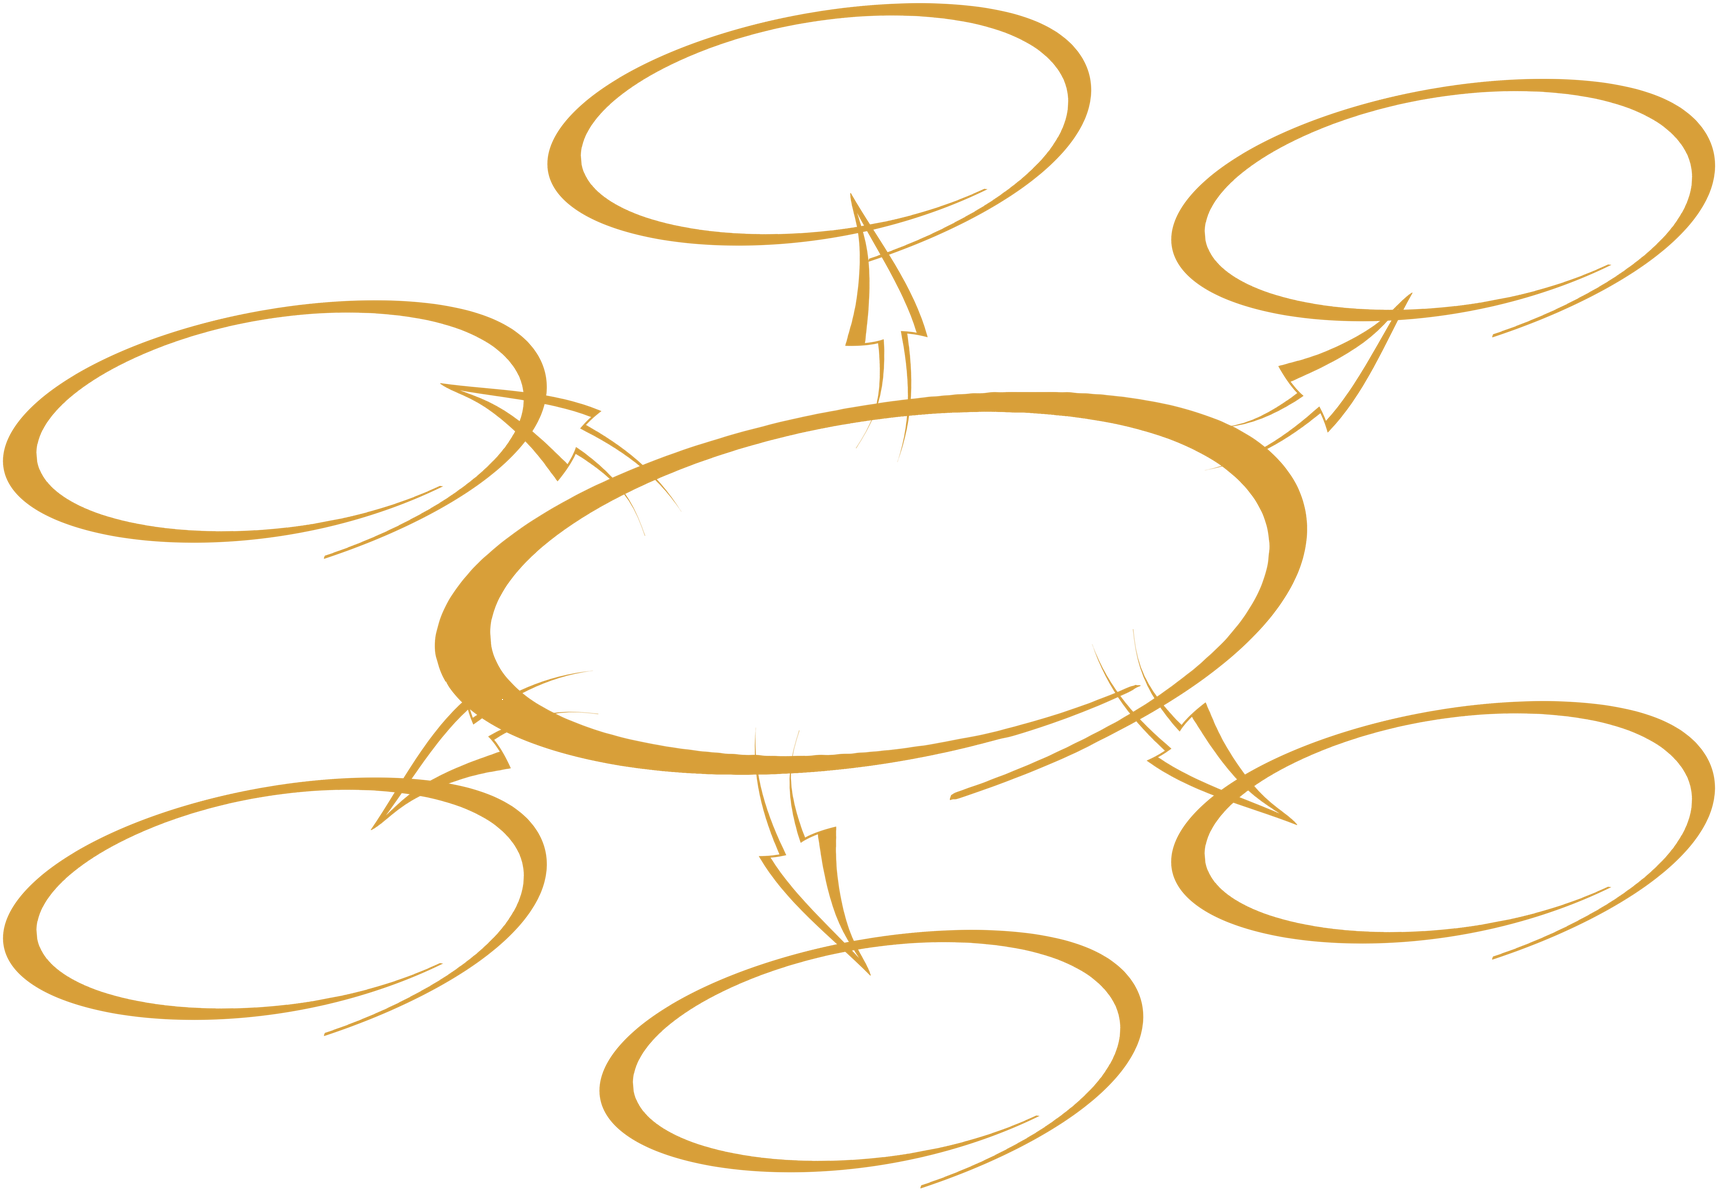
\includegraphics[height=2cm]{a30.png}    % The printed column  
\caption{Archaelogy 3.0 Symbol, pixabay [Pixabay License]}  % width is 8.4 cm.
\label{figa30symbol}                                 % Size the figures 
\end{center}                                 % accordingly.
\end{figure}

Lorem ipsum dolor sit amet, consetetur sadipscing elitr, sed diam nonumy eirmod tempor invidunt ut labore et dolore magna aliquyam erat, sed diam voluptua. At vero eos et accusam et justo duo dolores et ea rebum. Stet clita kasd gubergren, no sea takimata sanctus est Lorem ipsum dolor sit amet. Lorem ipsum dolor sit amet, consetetur sadipscing elitr, sed diam nonumy eirmod tempor invidunt ut labore et dolore magna aliquyam erat, sed diam voluptua. At vero eos et accusam et justo duo dolores et ea rebum. Stet clita kasd gubergren, no sea takimata sanctus est Lorem ipsum dolor sit amet. Lorem ipsum dolor sit amet, consetetur sadipscing elitr, sed diam nonumy eirmod tempor invidunt ut labore et dolore magna aliquyam erat, sed diam voluptua. At vero eos et accusam et justo duo dolores et ea rebum. Stet clita kasd gubergren, no sea takimata sanctus est Lorem ipsum dolor sit amet. 

\cite{bernerslee_linkeddata}

\cite{hausenblas_5star}

\cite{isaksen_archaeology}

\cite{thiery_geinarfa}

\begin{figure}[!htb]
\begin{center}
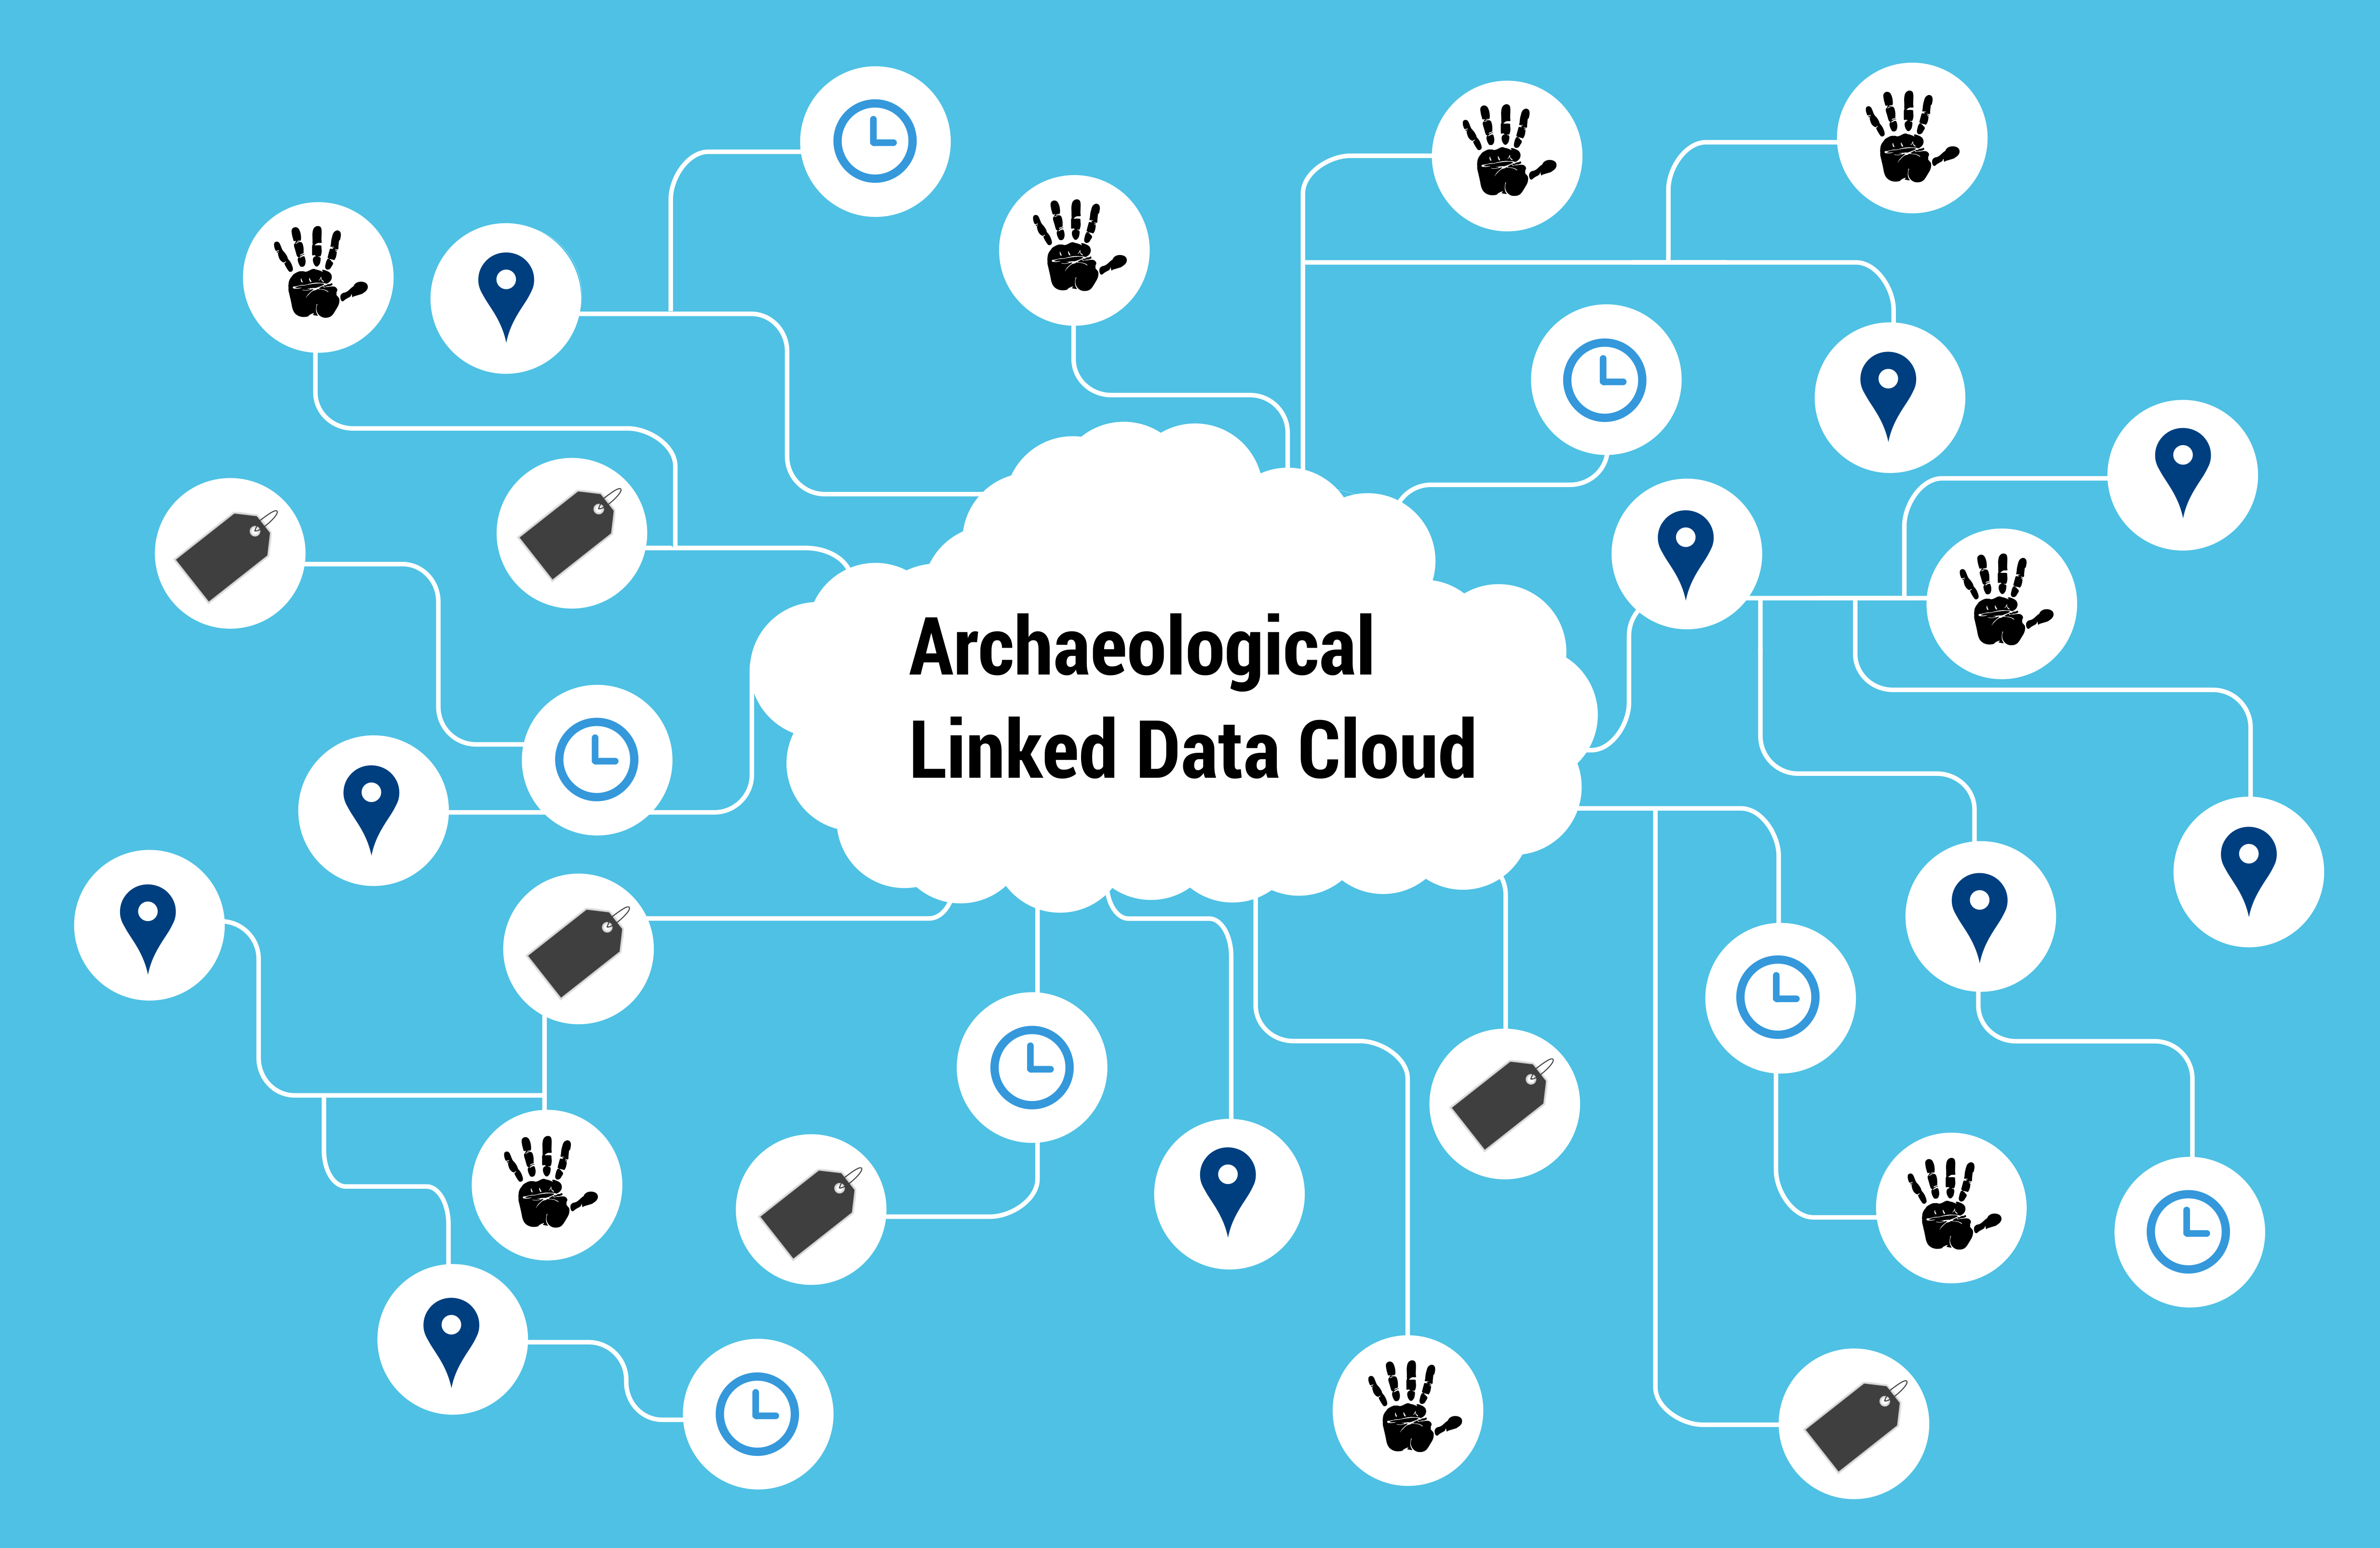
\includegraphics[width=8cm]{Archaeological_Linked_Data_Cloud_(ALDC).png}    % The printed column  
\caption{Archaeological Linked Data Cloud, Florian Thiery [CC BY 4.0]}  % width is 8.4 cm.
\label{figaaldc}                                 % Size the figures 
\end{center}                                 % accordingly.
\end{figure}

\begin{figure}[!htb]
\begin{center}
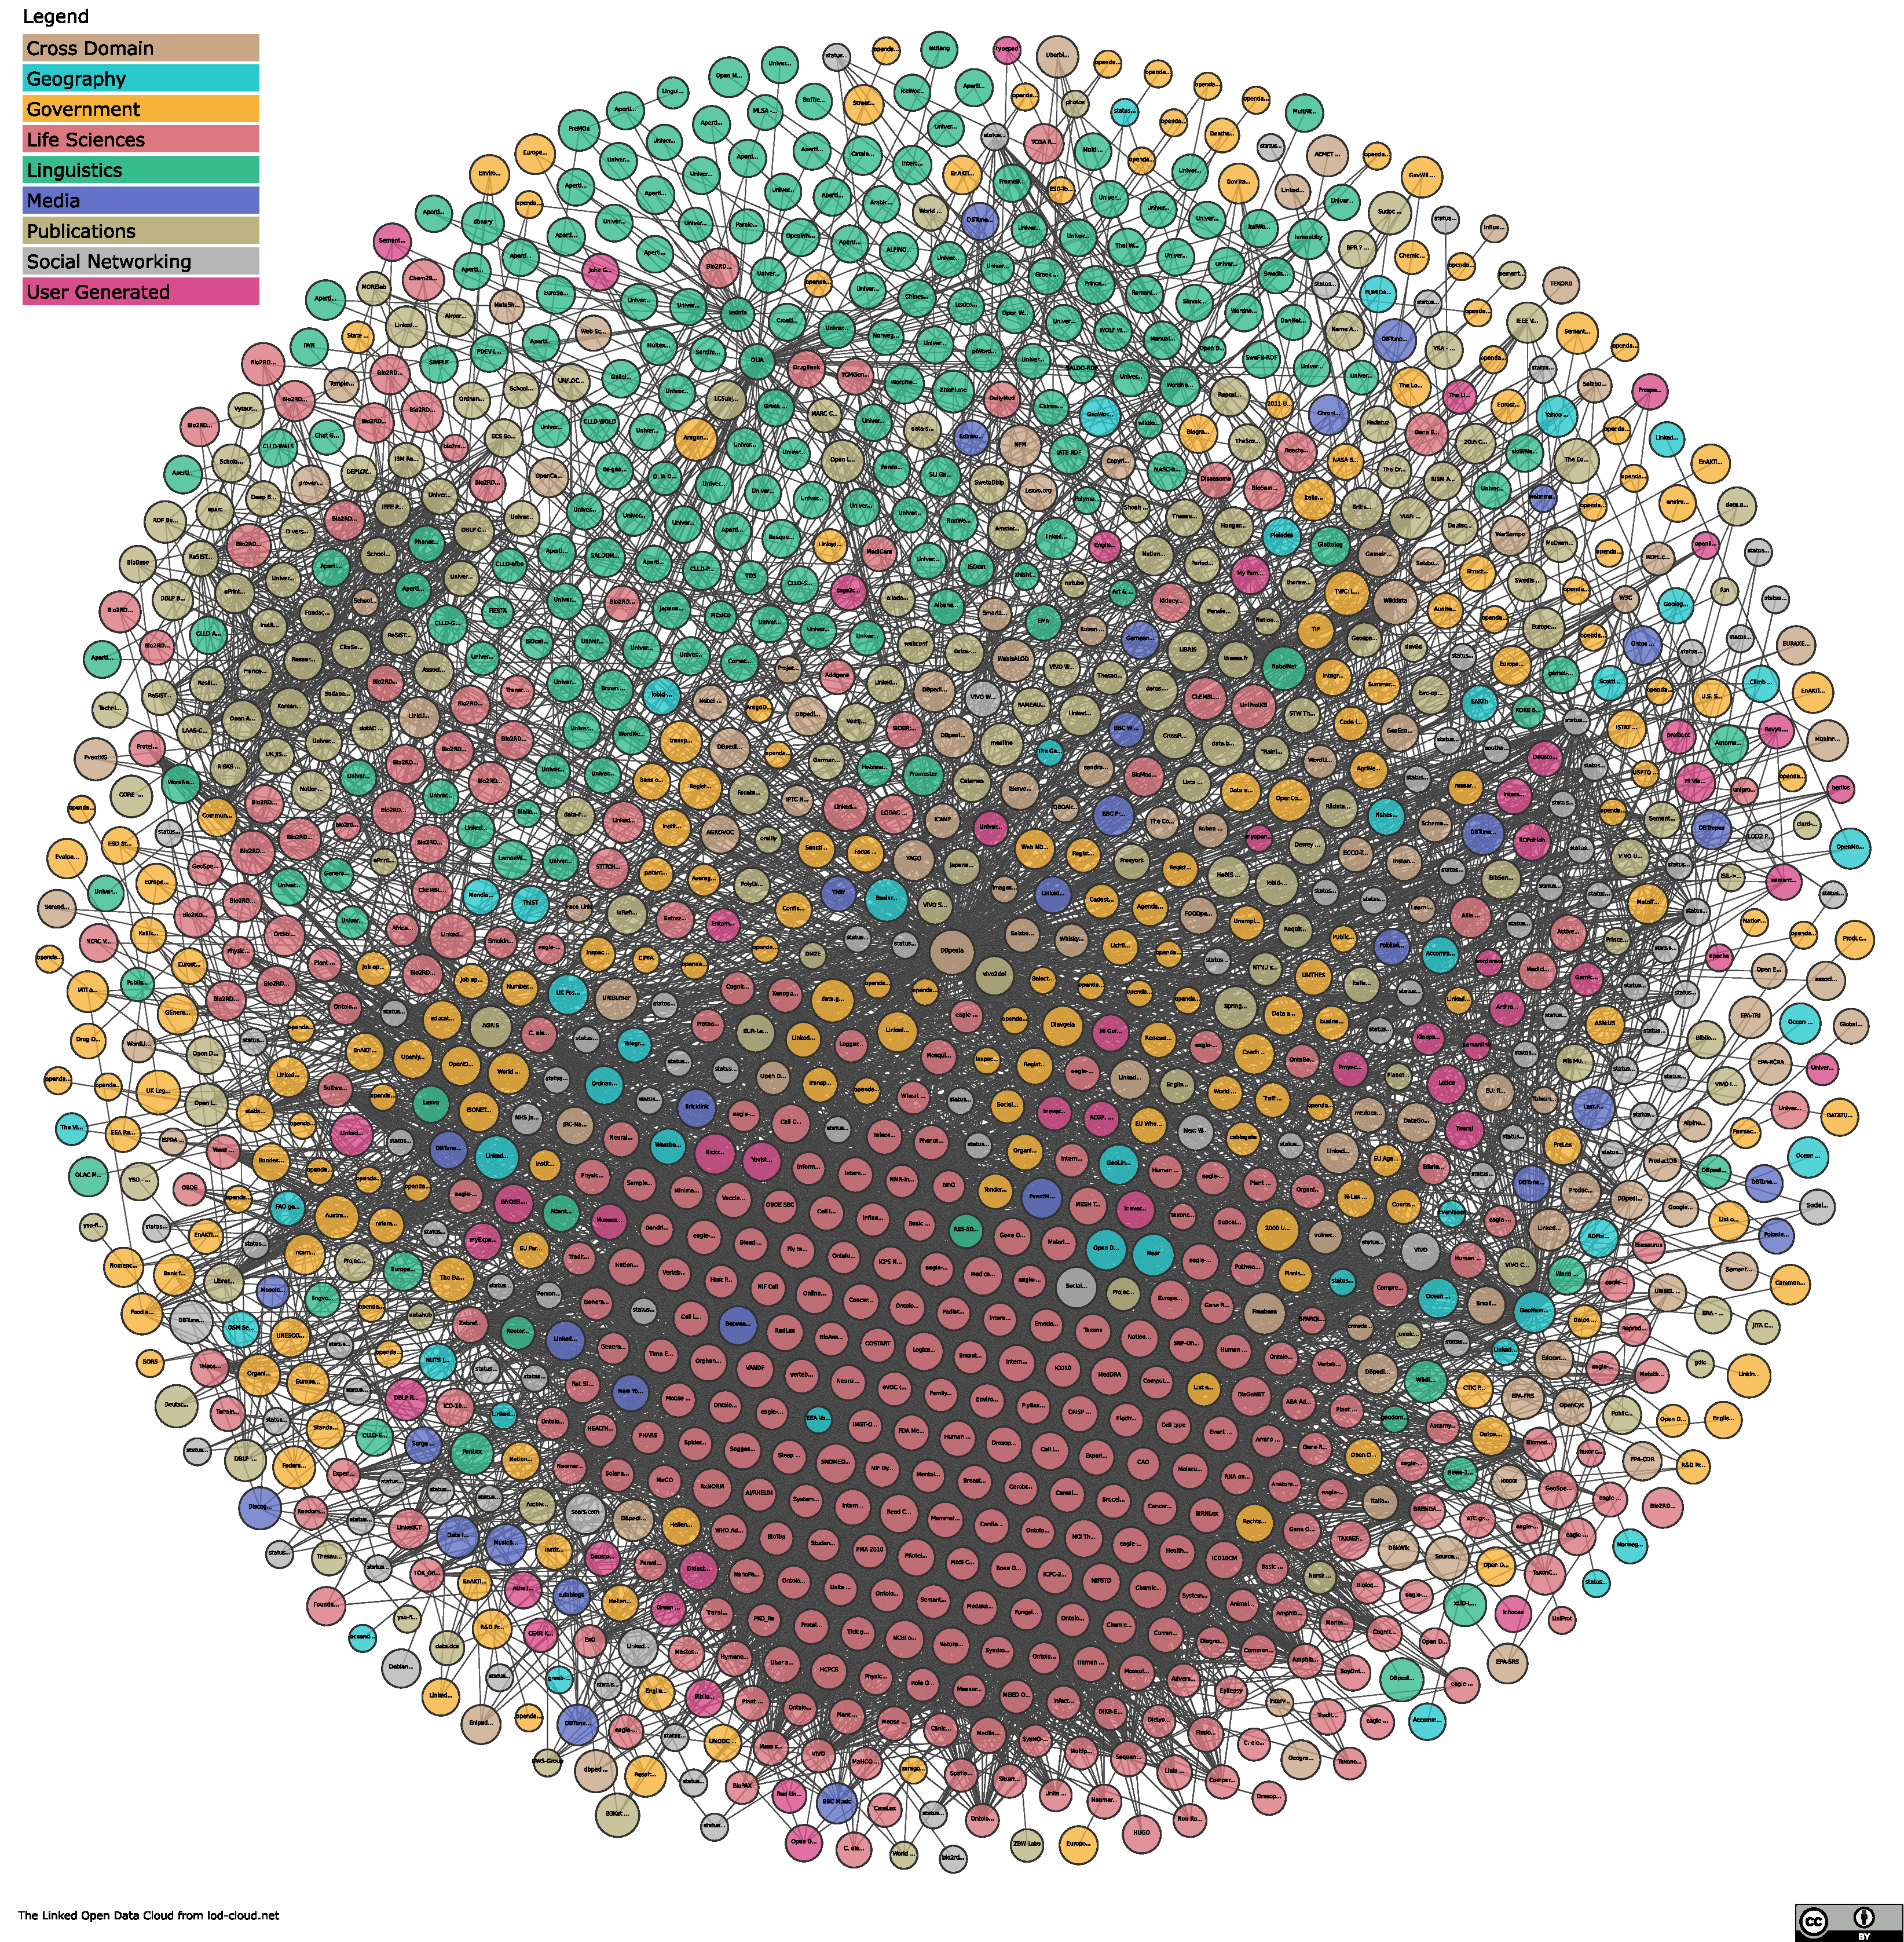
\includegraphics[width=8cm]{lod-cloud.pdf}    % The printed column  
\caption{Linked Open Data Cloud 2019-03-29, lod-cloud.net [CC BY 4.0]}  % width is 8.4 cm.
\label{figlodc}                                 % Size the figures 
\end{center}                                 % accordingly.
\end{figure}

\subsection{Archaeology 4.0}

\begin{figure}[!htb]
\begin{center}
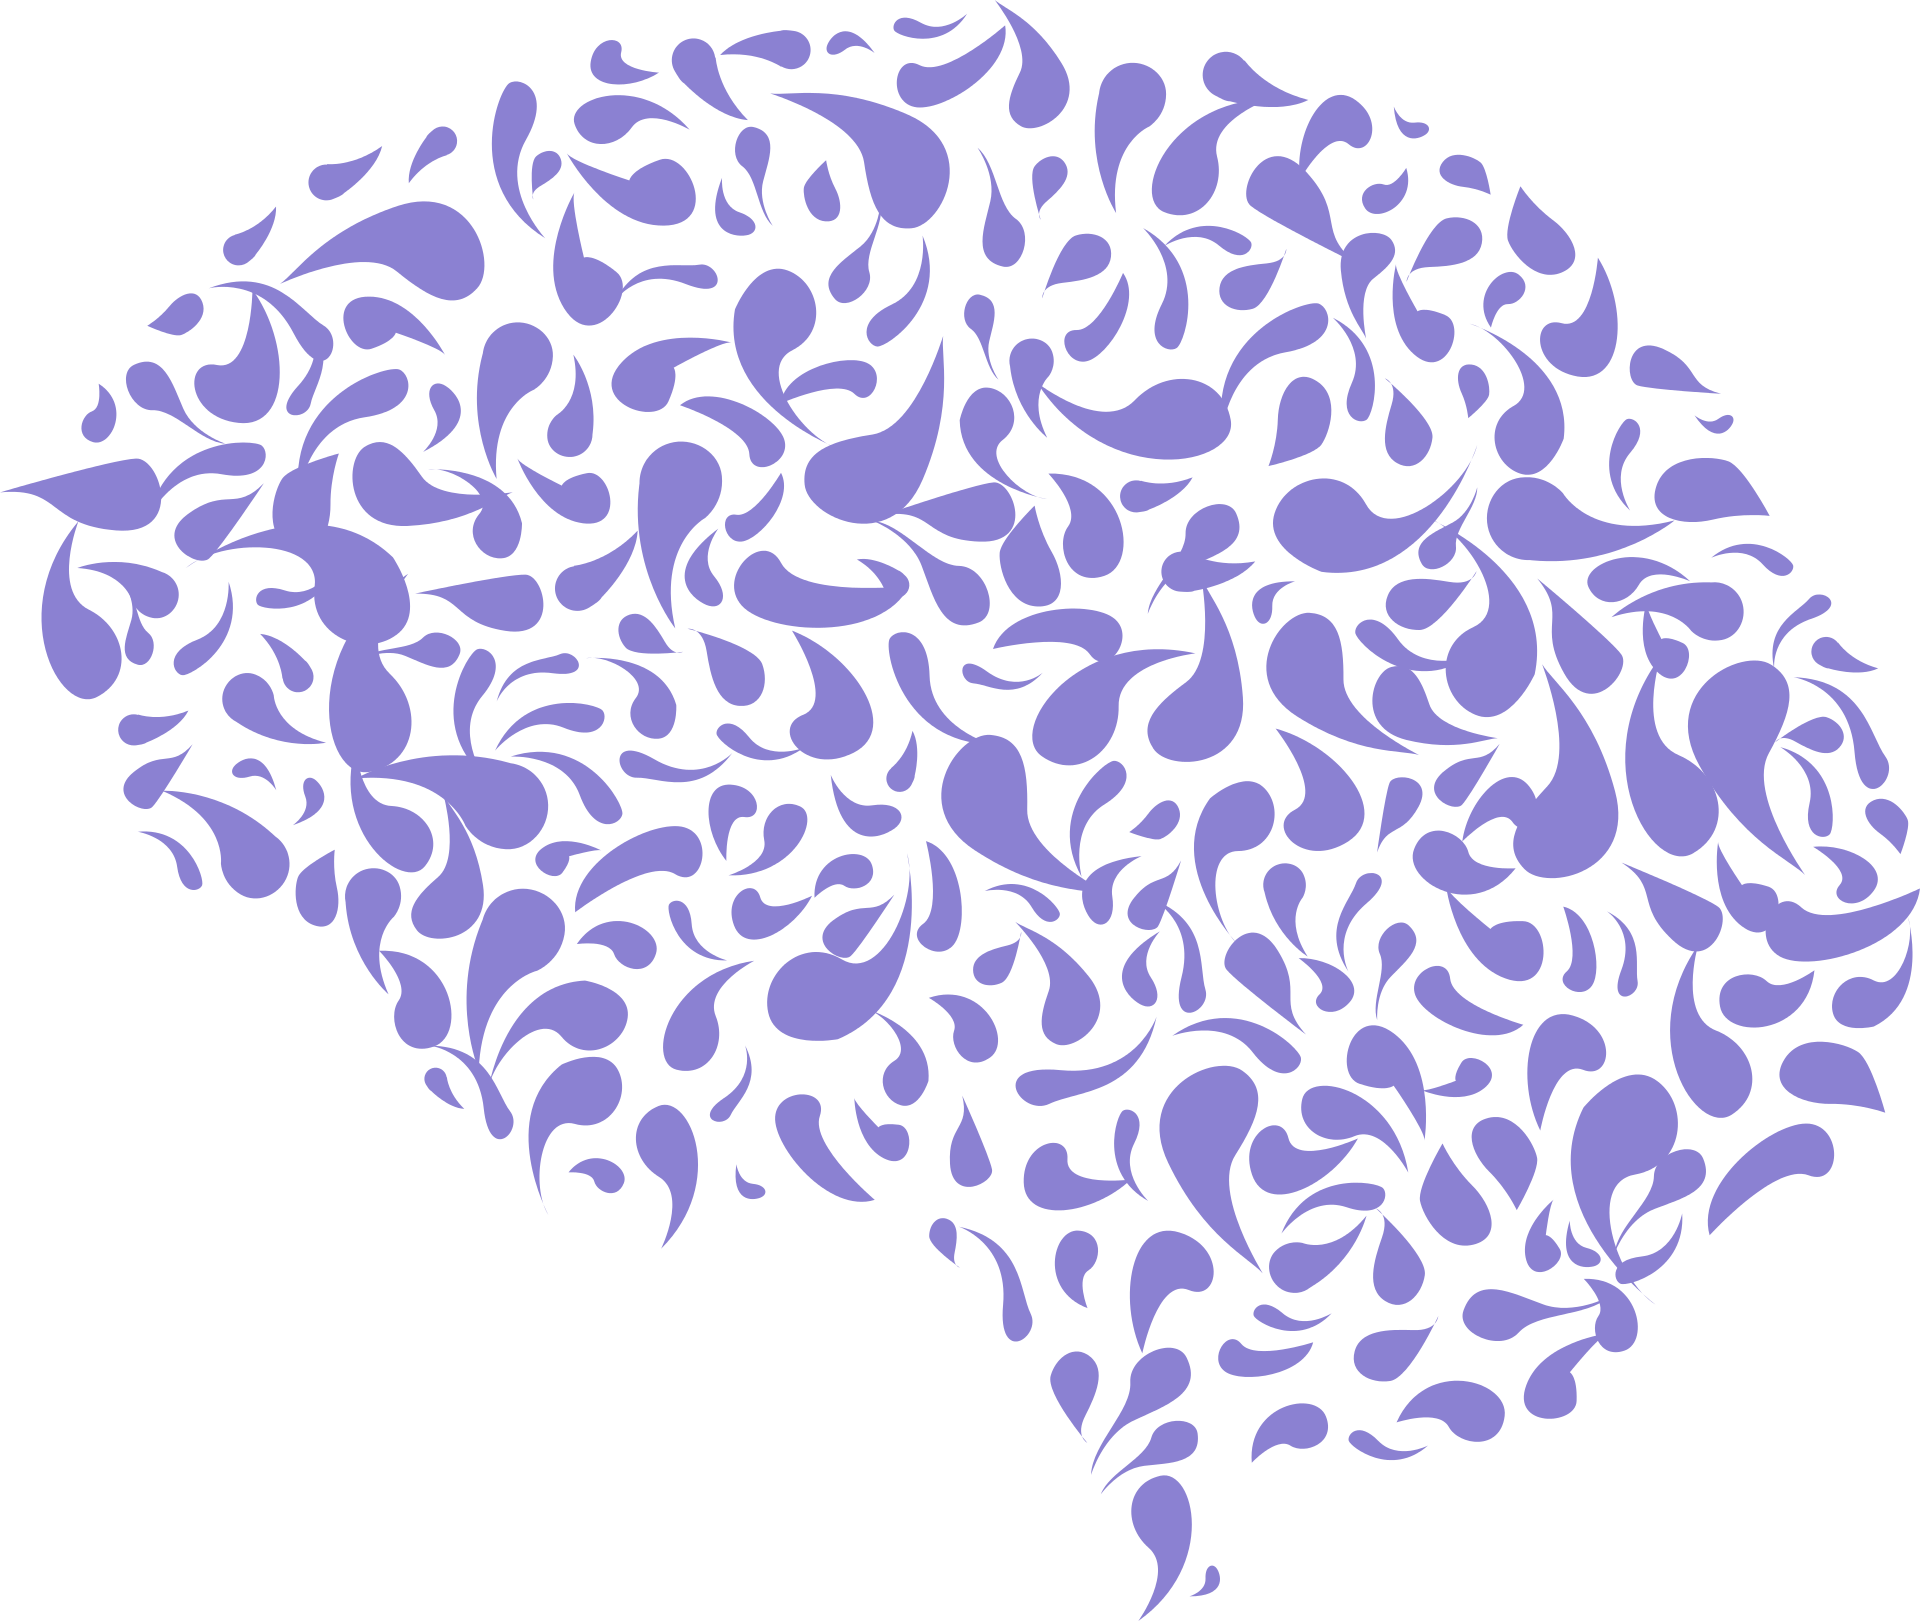
\includegraphics[height=2cm]{a40.png}    % The printed column  
\caption{Archaelogy 4.0 Symbol, pixabay [Pixabay License]}  % width is 8.4 cm.
\label{figa40symbol}                                 % Size the figures 
\end{center}                                 % accordingly.
\end{figure}

Lorem ipsum dolor sit amet, consetetur sadipscing elitr, sed diam nonumy eirmod tempor invidunt ut labore et dolore magna aliquyam erat, sed diam voluptua. At vero eos et accusam et justo duo dolores et ea rebum. Stet clita kasd gubergren, no sea takimata sanctus est Lorem ipsum dolor sit amet. Lorem ipsum dolor sit amet, consetetur sadipscing elitr, sed diam nonumy eirmod tempor invidunt ut labore et dolore magna aliquyam erat, sed diam voluptua. At vero eos et accusam et justo duo dolores et ea rebum. Stet clita kasd gubergren, no sea takimata sanctus est Lorem ipsum dolor sit amet. Lorem ipsum dolor sit amet, consetetur sadipscing elitr, sed diam nonumy eirmod tempor invidunt ut labore et dolore magna aliquyam erat, sed diam voluptua. At vero eos et accusam et justo duo dolores et ea rebum. Stet clita kasd gubergren, no sea takimata sanctus est Lorem ipsum dolor sit amet. 

\cite{mccreary_computing}

\cite{hey_computing}

\begin{figure}[!htb]
\begin{center}
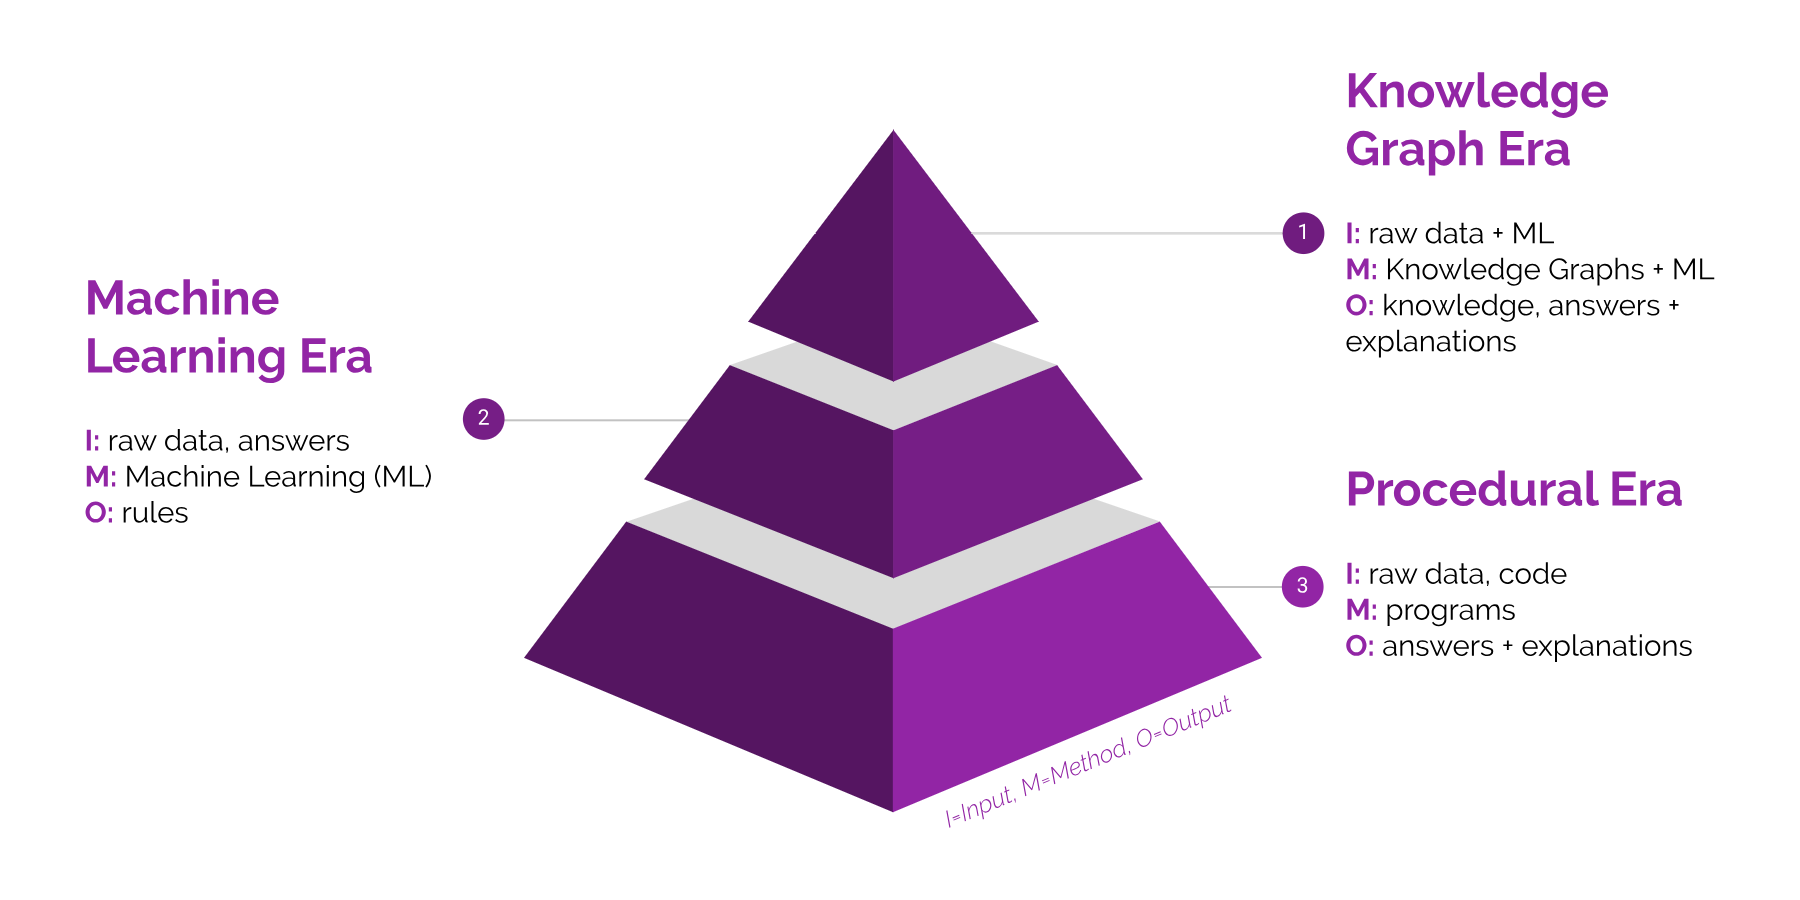
\includegraphics[width=8cm]{Era_of_Computing.png}    % The printed column  
\caption{Era of Computing, Florian Thiery [CC BY 4.0]}  % width is 8.4 cm.
\label{figeoc}                                 % Size the figures 
\end{center}                                 % accordingly.
\end{figure}

\begin{figure}[!htb]
\begin{center}
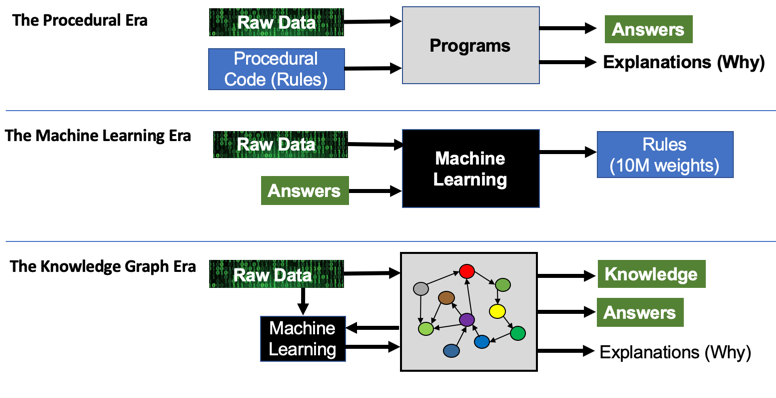
\includegraphics[width=8cm]{1_78b9DR1EApGRAst5FkPrwQ.png}    % The printed column  
\caption{Era of Computing, Dan McCreary \cite{mccreary_computing}}  % width is 8.4 cm.
\label{figeoco}                                 % Size the figures 
\end{center}                                 % accordingly.
\end{figure}

\begin{ack}                               
I would like to thank the Mainz Centre for Digitality in the Humanities and Cultural Studies (mainzed) and R\"omisch-Germanisches Zentralmuseum. In particular Prod. Dr. Kai-Christian-Bruhn (ORCID: 0000-0001-8322-1260) and Dr. Allard Mees FSA (ORCID: 0000-0002-7634-5342).
\end{ack}

\bibliographystyle{plain}        % Include this if you use bibtex 
\bibliography{autosam}           % and a bib file to produce the 
                                 % bibliography (preferred). The
                                 % correct style is generated by
                                 % Elsevier at the time of printing.

\end{document}